
In this section, we first introduce the basic assumptions underlying our approach (Section \ref{sec:assumption-causal}), then we present our proposed end-to-end approach for anomaly detection and root cause analysis, namely BARO (Sections \ref{sec:approach-ovw}, \ref{sec:multi-bocpd}, \ref{sec:robustscorer}). \textbf{BARO} incorporates a Multivariate \textbf{BA}yesian Online Change Point Detection technique to model the dependency and correlation structure of multivariate time series metrics data, enabling it to effectively detect anomalies and estimate the occurrence time of failures
(Section \ref{sec:multi-bocpd}). Then it uses a nonparametric hypothesis testing method, referred to as \textbf{RO}bustScorer, to reliably identify and rank the potential root causes, which is less sensitive to the accuracy of the anomaly detection time (Section \ref{sec:robustscorer}). 


 
\subsection{Basic Assumptions} \label{sec:assumption-causal}

\subsubsection{Anomaly Metrics} \label{sec:anomaly-metric-selection}

As commonly recognized in previous works \cite{Li2022Circa, yu2023cmdiagnostor, liu2021microhecl}, there are generally four types of metrics: \textit{Traffic} (e.g., request count per minute), \textit{Saturation} (e.g., CPU utilization, database records), \textit{Latency} (e.g., average response time per minute), and \textit{Errors} (e.g., the rate of failed requests). These four types are named after the four golden signals in site reliability engineering \cite{googlesre}. Following the practice in metric-based RCA studies \cite{yu2023cmdiagnostor, Xin2023CausalRCA, Jinjin2018Microscope, Li2022Circa, Azam2022rcd}, we assume that \textit{anomalies should be visible in the metrics, subsequently affecting \textit{Latency} and/or \textit{Errors}.} With these assumptions, in varying conditions where there is a surge in \textit{Traffic} or \textit{Saturation} (e.g., in holiday periods) but without abnormal increases in \textit{Latency} and \textit{Errors}, our proposed method considers these situations as normal. Conversely, if a surge in \textit{Traffic} or \textit{Saturation} metrics causes abnormal increases in \textit{Latency} or \textit{Errors}, our method considers this an anomaly. Finally, for the RCA task, our method considers all the metrics to pursue the fine-grained output root cause ranking.


\subsubsection{Failure Propagation Chain} \label{sec:assumption-failure-propagation}

In practice, when a service failure occurs, it generally results in an anomaly in the data associated with the metric corresponding to that failure~\cite{Li2022Circa, Azam2022rcd}. For example, network congestion in a service typically leads to an increase in its response time. Furthermore, since a failure can propagate across the services within the system, this initial anomaly will then trigger additional anomalies in the metrics data of other services at later time~\cite{Azam2022rcd, Xin2023CausalRCA, Jinjin2018Microscope, Li2022Circa, liu2021microhecl}. Thus, when an anomaly is detected and the RCA module is activated, the anomalous period of runtime metrics data generally consists of multiple anomalies. In this work, based on this failure propagation chain, we assume \textit{the first anomaly corresponds to the time when the failure first occurs}. Thus, in our proposed method, we use the first detected anomaly to approximate the failure occurrence time ($\hat{t}_A$ in Alg. \ref{alg:baro}) to separate the normal and abnormal metrics data. It is important to note that this assumption does not imply the first detected anomaly to be the root cause, and, it has been implicitly used in previous RCA works \cite{Shan2019Ediagnosis, Li2022Circa, Azam2022rcd} for the same purpose as ours (i.e. to separate the abnormal and normal data). Our experimental results, along with those of previous studies, affirm the validity of this assumption.


\begin{figure}[t]
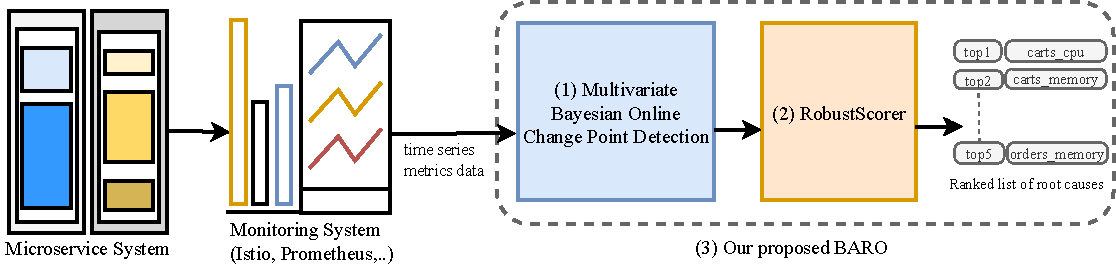
\includegraphics[width=\textwidth]{image/intro6.drawio.pdf}
\vspace{-0.5cm}
\caption{The overview: The monitoring system monitors the microservice system and collects the time series data. Our BARO consists of two components: Multivariate BOCPD and RobustScorer. The Multivariate BOCPD acts as an anomaly detection module to continuously check whether there is an anomaly. If there exists an anomaly, it triggers RobustScorer to score and rank the root cause services and metrics correspondingly.} \label{fig:intro2}
\end{figure}

\subsection{Approach Overview} \label{sec:approach-ovw}

We illustrate BARO, our proposed end-to-end approach for anomaly detection and root cause analysis for microservice systems based on multivariate time series metrics data, in Fig. \ref{fig:intro2}. BARO consists of two main components. The first component is a Multivariate Bayesian Online Change Point Detection (BOCPD) module to model the dependency and correlation structure of multivariate time-series metrics data so as to detect anomalies (failures). The second component is Robust Scorer, a nonparametric statistical hypothesis testing technique to identify the root cause associated with the failures. Thus, the outputs of BARO include: (1) a boolean indicating whether an anomaly is presented, (2) a ranked list of root cause metrics and their corresponding services, with the highest-ranked items having the highest probability of being the root cause of the failure, if an anomaly is detected. The pseudocode of BARO is described in Algorithm \ref{alg:baro}.


\subsection{Multivariate Bayesian Online Change Point Detection} \label{sec:multi-bocpd}

Anomaly detection in microservices involves identifying anomalies, i.e., observable symptoms of failures \cite{Soldani2022rcasurvey}, while failures in microservices can be considered as interventions that change the monitoring data distribution \cite{Azam2022rcd, Li2022Circa}. Therefore, to detect anomalies (failures) within microservices via time series metrics data, we formulate this problem as a change point detection problem whose goal is to identify whether the behavior of a time series changes significantly. We then propose to use Multivariate BOCPD, a combination of BOCPD \cite{adams2007bayesian} and MultivariateCPD \cite{xuan2007modeling}, to model the dependency and correlation among metrics to detect anomalies effectively. The motivation behind this design is twofold. First, we propose to use BOCPD \cite{adams2007bayesian} as a base technique for detecting change points as it is a simple yet effective online detection technique and it requires no user-specified thresholds to identify change points for univariate time series. It has been shown to be among the best current change point detection methods in many real-world scenarios \cite{Burg2022CPeval}. Second, by combining BOCPD with MultivariateCPD \cite{xuan2007modeling}, we can model the structure and dependency among the multivariate time series metrics data better. This is especially useful for detecting anomalies within microservices due to the failure propagation chain in microservices described in Section \ref{sec:assumption-failure-propagation}. Specifically, anomalies in microservices are generally propagated across the metrics data, causing correlated and dependent changes among different time series metrics. MultivariateCPD has been shown to be able to effectively detect change points when the changes occur in the correlation structure as in multivariate time series metrics data. In the following paragraphs, we describe in detail these two components of our proposed method.



The main idea of BOCPD is to model the \textit{run length}, i.e. the number of consecutive data points in the same distribution, since the last change point, given the data observed so far. Specifically, the run length $r_t$ at time $t$ is defined as $0$ if there is a change point at time $t$, and as $r_{t-1}+1$ otherwise. Given the time series metrics data $\mathcal{M}^{i,j=1:n,1:m}_{t_0:t}$, using the Bayes theorem, the posterior probability distribution of the run length $p(r_t \vert \mathcal{M}^{i=1:n,j=1:m}_{t_0:t})$ can be computed as \cite{adams2007bayesian},
\begin{equation} \label{eq:bocpd-run-length}
    p(r_t \vert \mathcal{M}^{i,j=1:n,1:m}_{t_0:t}) = \frac{\sum\nolimits_{r_{t-1}} p(r_t \vert r_{t-1}) p(\mathcal{M}^{i,j=1:n,1:m}_{t} \vert r_{t-1}, (\mathcal{M}^{i,j=1:n,1:m}_{t})^{(r)}) p(r_{t-1} \vert \mathcal{M}^{i,j=1:n,1:m}_{t_0:t-1})} {p(\mathcal{M}^{i,j=1:n,1:m}_{t_0:t})},
\end{equation}
where $(\mathcal{M}^{i,j=1:n,1:m}_{t})^{(r)}$ denotes the set of observed data points associated with the run $r_t$. The formula in Eq. (\ref{eq:bocpd-run-length}) is recursive, meaning that we can compute the posterior distribution of the run length $r_t$ based on the posterior distribution of $r_{t-1}$, the conditional prior of run length $p(r_t \vert r_{t-1})$ and the distribution of the metrics data $p(\mathcal{M}^{i,j=1:n,1:m}_{t_0:t})$. As suggested in \cite{adams2007bayesian}, the marginal likelihood of the metrics data $p(\mathcal{M}^{i,j=1:n,1:m}_{t_0:t})$ can be chosen as a distribution from the exponential family and the conditional prior of run length $p(r_t \vert r_{t-1})$ can be set based on a hazard function with discrete exponential (geometric) distribution. At each time step $t$, the most probable run length is computed as the value with the highest probability $p(r_t \vert \mathcal{M}^{i,j=1:n,1:m}_{t_0:t})$. Finally, the change points are identified as the data points at the time steps whose run lengths decrease.


The main idea of MultivariateCPD, given the time series metrics data $\mathcal{M}^{i,j=1:n,1:m}_{t_0:t_0+T}$, is to model the metrics data at each data point $\mathcal{M}^{i,j=1:n,1:m}_t$ using a multivariate model \cite{xuan2007modeling}. A common choice is to use the multivariate Gaussian, i.e., $\mathcal{M}^{i,j=1:n,1:m}_t \sim \mathcal{N}(0, \Sigma)$, with $\Sigma$ is an inverse Wishart prior $\Sigma \sim IW(N_0, V_0)$ and $N_0$ is set to be $mn$ which is the number time series within the metrics dataset and $V_0$ is set to be $\hat{\sigma}^2 I$, $I$ is the identity matrix and $\hat{\sigma}$ is the mean of the empirical variance pooled across all the metrics data. With this formulation, let us denote $h=(t_2-t_1)+1$, the marginal likelihood of the multivariate time series data $\mathcal{M}^{i,j=1:n,1:m}_{t_1:t_2}$ can then be computed explicitly as~\cite{xuan2007modeling},
\begin{equation}
\begin{aligned}
p(\{\mathcal{M}^{i,j=1:n,1:m}_{t_1:t_2}\}) &= \pi^{-\frac{hmn}{2}} \frac{\vert V_0 \vert^{N_0/2}}{\vert V_h\vert^{(N_0+h)/2}}  \frac{\Gamma_{mn}(N_0/2)^{-1}}{\Gamma_{mn}((N_0+h)/2)^{-1}}, \\
V_h &= V_0 + S, S=\sum_{i=t_1}^{t_2}  \mathcal{M}^{i,j=1:n,1:m}_t {\big(\mathcal{M}^{i,j=1:n,1:m}_t\big)}^\intercal,
\end{aligned}
\end{equation}
where $\Gamma_{mn}(.)$ denotes the multivariate gamma function. This formulation of the marginal likelihood $p(\mathcal{M}^{i,j=1:n,1:m}_{t_1:t_2})$ can then incorporated into Eq. (\ref{eq:bocpd-run-length}) to replace the univariate marginal likelihood. Other steps are kept the same in order to detect change points in the time series metrics data.

Fig. \ref{fig:mbocpd} presents two examples of using Multivariate BOCPD to detect change points within multivariate time series metrics data using two different datasets. It can be seen that Multivariate BOCPD can accurately detect change points (data points that separate the normal and abnormal data), and thus, detect the failures.

Finally, note that following the assumptions in Section \ref{sec:assumption-causal}, we use \textit{Latency} and \textit{Errors} to detect anomalies, and we only output the first detected change point as the detected anomaly.



\begin{figure}[t]
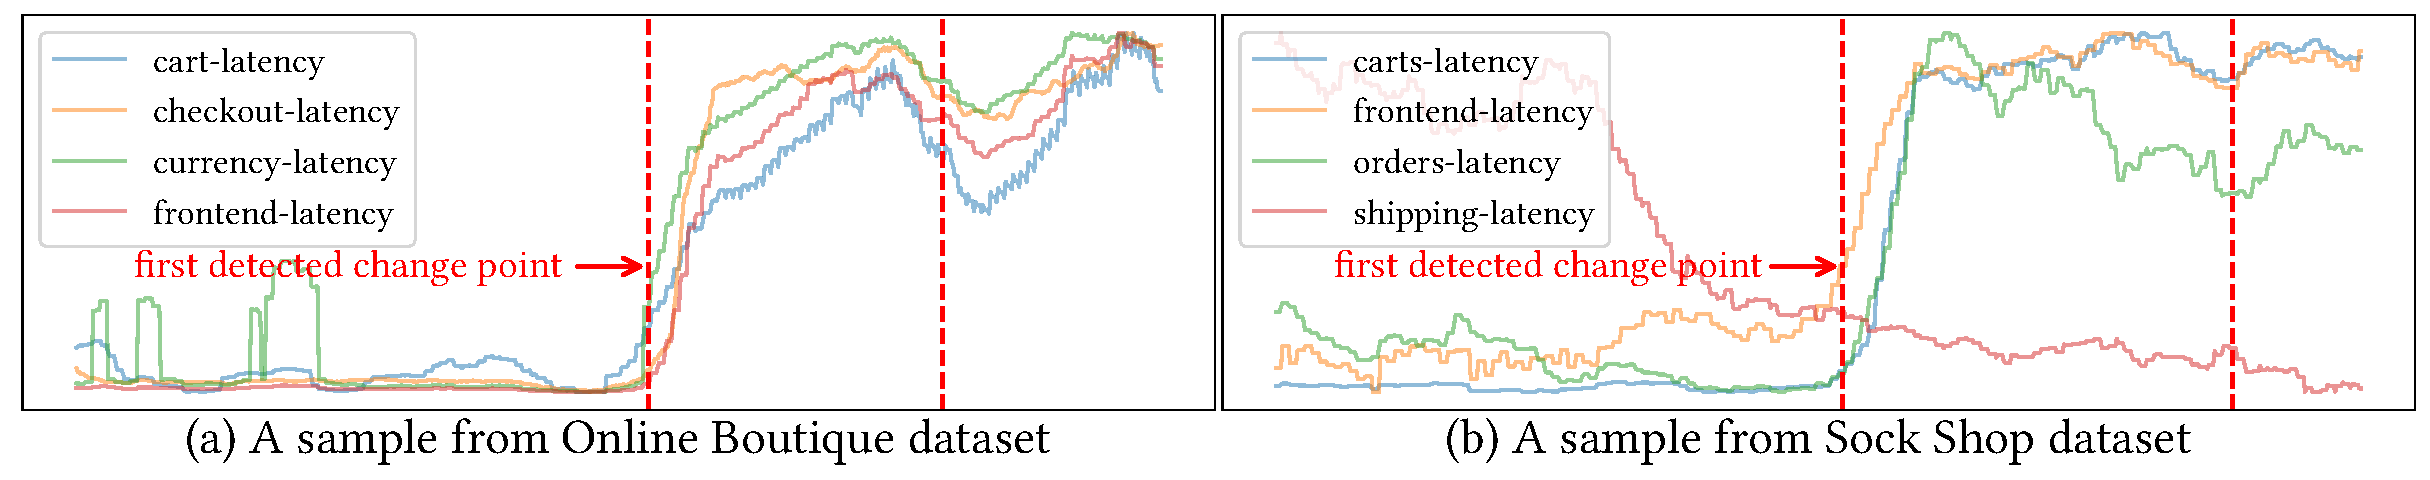
\includegraphics[width=0.97\textwidth]{image/bocpd_visualize.pdf}
\vspace{-0.2cm}
\caption{An example of using Multivariate BOCPD to detect change points on multivariate time series data. \textcolor{red}{Dotted vertical red lines} indicate change points. We observe that Multivariate BOCPD can provide the anomaly detection time (the first change point) accurately that separate the normal and abnormal period. In the abnormal period there are multiple change points due to the failure propagation chain.} 
\label{fig:mbocpd}
\vspace{-0.1cm}
\end{figure}







\begin{algorithm}[hbt!]
\caption{Pseudo-code of BARO} \label{alg:baro}
\begin{algorithmic}[1]
\Require a set of metrics data $\mathcal{M} = \{x^{i=1:n,j=1:m}_{t_0:t_0+T}\}$ 
\Ensure ranked candidate root causes $\mathcal{R}$, ($\mathcal{R} \in \mathcal{M}$) if detected anomaly

\Function{MultivariateBOCPD}{$\mathcal{M}$}
  \State $\mathcal{M}' \gets$ 
 select \textit{Latency} and \textit{Errors} from $\mathcal{M}$
  \State compute the run length probability $p(r_t \vert \{\mathcal{M'}_{t_0:t}\})$, $\forall x^{(i,j)}\in \mathcal{M'}$, $\forall t\in [t_0, t_0 + T]$
  \State $s_t \gets$ argmax $p(r_t \vert \{\mathcal{M'}_{t_0:t}\}$, $\forall t\in [t_0, t_0 + T]$
  \For{$t\in [t_0, t_0 + T]$} 
    \If {$s_t \le s_{t - 1}$} 
      \State \Return $y = 1, \hat{t}_A = t$; \quad // Returns anomaly if there is a change point detected 
    \EndIf  
  \EndFor   
  \State \Return $y=0,\hat{t}_A=nul$; \quad // Returns normal if there is no change point detected
\EndFunction

\Function{RobustScorer}{$\mathcal{M}$, $\hat{t}_A$}
  \State $\mathcal{R} \gets$ empty list
  \For{$x^{(i, j)} \in \mathcal{M}$}
    \State $\rho^{(i,j)} \gets 0$; med, IQR $\gets$ learn from $\{x^{(i,j)}_{t'}\}$, where $t_0 \le t' \le \hat{t}_A$ 
    \For{$t''$ from $\hat{t}_A$ to $t_{0} + T$}
        \State $a^{(i,j)}_{t''}$ = abs($x^{(i,j)}_{t''}$ - med) / IQR; $\rho^{(i,j)} = \max(\rho^{(i,j)}, a^{(i,j)}_{t''})$
    \EndFor 
    \State $\mathcal{R} \gets \mathcal{R}$ appends ($x^{(i,j)}$, $\rho^{(i,j)}$)
  \EndFor 
  \State $\mathcal{R} \gets$ reversely sort $\mathcal{R}$ based on $\rho^{(i,j)}$
  \State \Return $\mathcal{R}$
\EndFunction

\Procedure{BARO}{$\mathcal{M}$}
  \State $y, \hat{t}_A \gets$ \Call{MultivariateBOCPD}{$\mathcal{M}$} \quad // Step 1: Run Multivariate BOCPD
  
  \State \Return \Call{RobustScorer}{$\mathcal{M}$, $\hat{t}_A$} \textbf{if} $y=1$ \textbf{else} \Return nul // Step 2: Run RobustScorer with $\hat{t}_A$
  
\EndProcedure 
\end{algorithmic}
\end{algorithm}


\subsection{RobustScorer: A Robust Nonparametric Hypothesis Testing Technique} \label{sec:robustscorer}

To identify the root cause metrics, we aim to identify the metrics that exhibit significant changes in data distribution at the anomaly detection time \cite{Shan2019Ediagnosis, liu2023pyrca, Li2022Circa}. To solve this problem, one approach is to conduct hypothesis testing and test whether the data distribution of the metrics data changes significantly after the anomaly detection time. This approach was employed in $\epsilon$-Diagnosis \cite{Shan2019Ediagnosis, liu2023pyrca} and NSigma \cite{Li2022Circa} and they have been shown to perform very well in various scenarios. Our key insight is that previous works might be extremely sensitive to the anomaly detection output (failure occurrence time $\hat{t}_A$), i.e., inaccurate specification of the failure occurrence time might yield bad root cause analysis. Therefore, we propose RobustScorer to address this problem.

Specifically, for each metric $x_{t_0:t_0+T}^{(i,j)}$ in the metrics dataset $\mathcal{M}^{i,j=1:n,1:m}_{t_0:t_0+T}= \{x^{i=1:n,j=1:m}_{t_0:t_0+T}\}$, we conduct a hypothesis test based on the following null hypothesis ($\textbf{H}_0$):\textit{ $x^{(i,j)}$ is not a root cause metric for the failure}. This null hypothesis means that, for $t$ after the anomaly detection time, $x^{(i,j)}_t \sim \mathcal{L}(x^{(i,j)}_{t_\text{normal}})$ with $\mathcal{L}(x^{(i,j)}_{t_\text{normal}})$ denoting the distribution of the metrics data during the normal period (when $t$ is before the anomaly detection time).


This approach generally requires the specification of the anomaly detection time. Inaccurate anomaly detection time therefore could impact the accuracy of these techniques significantly. In this section, we propose a novel nonparametric hypothesis testing technique that is robust and less sensitive to the accuracy of the anomaly detection time.


\subsubsection{A Robust Nonparametric Hypothesis Test}

RobustScorer follows a statistical approach to learn the expected distribution from the metrics data. For every time series $x^{(i,j)}_{t_0:t_0+T}$ in the metrics dataset $\mathcal{M}^{i,j=1:n,1:m}_{t_0:t_0+T}$, let us denote $\hat{t}_A$ as the anomaly detection time, which is an estimation of the time when the anomaly occurs, RobustScorer is trained using the data collected prior to the anomaly, spanning from $t_0$ to $\hat{t}_A$, to learn the median ($med$) and interquartile range ($IRQ$) of this data distribution. Subsequently, for each data point $x^{(i,j)}_t$ in the anomalous period (from $\hat{t}_A$ to $t_0+T$), RobustScorer measures how significant it deviates from the expected central tendency. This deviation is denoted as $a^{(i,j)}_t$ and is computed as follows,
\begin{equation} \label{eq:robust-scoring-1}
    a^{(i,j)}_t = \big | x^{(i,j)}_t - med \big | / IQR.
\end{equation}

All the values of $a^{(i,j)}_t$ across all the metrics data during the anomalous period are then consolidated to yield $\rho^{(i, j)}$, which is an indicator measuring the changes of each metric during the anomalous period,

\begin{equation} \label{eq:robust-scoring-2}
    \rho^{(i, j)} = \max_{\hat{t}_A \leq t \leq t_0+T} a^{(i, j)}_t.
\end{equation}


A higher $\rho^{(i, j)}$ signifies a greater likelihood that $x^{(i, j)}$ serves as the root cause metric, thereby identifying $s^i$ as the root cause service. Finally, RobustScorer then generates a ranked list of root cause metrics based on the magnitudes of $\rho^{(i, j)}$, 
arranged in descending order, with the highest ones corresponding to the most probable root cause metrics (fine-grained root causes). The coarse-grained ranked list of root cause services can be derived from the fine-grained ranking list by extracting the services corresponding to the metrics. Note that we do not use the p-value to reject/accept a possible root cause as in standard hypothesis testing. In our method, we use hypothesis testing to rank the potential root causes as it is normal for the system operators to focus on the top candidates.


Similar to \cite{Li2022Circa, Shan2019Ediagnosis}, our proposed RobustScorer is also distribution-free, scale-equivalent (i.e. metrics data in different scales do not affect the ranked list of root causes), and rotation-invariant (i.e. timestamp shifts do not affect the ranked list of root causes).



\begin{figure}[ht]
\centering
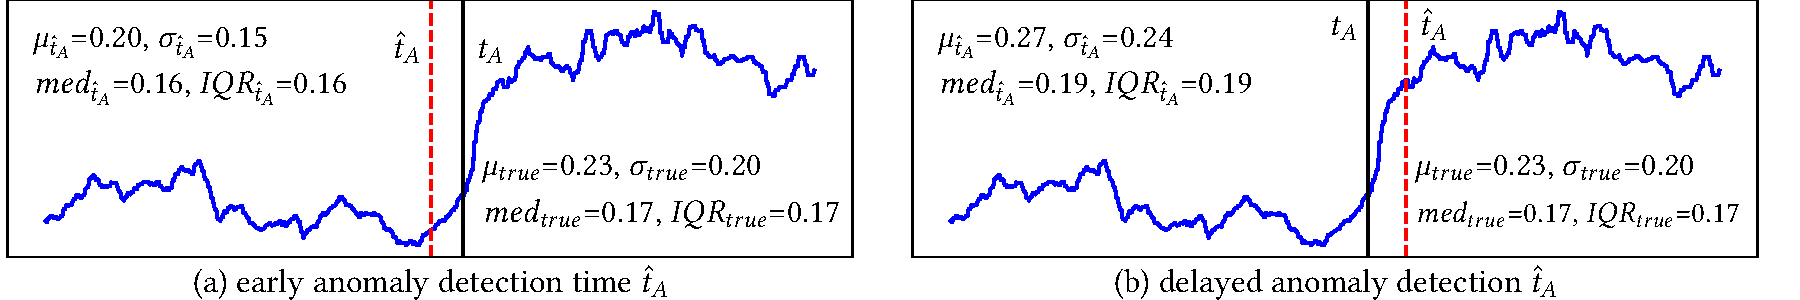
\includegraphics[width=0.98\textwidth]{image/method-iqr-robustness.pdf}
\vspace{-0.2cm}
\caption{The Robustness of RobustScorer against imprecise anomaly detection time. In (a), an early anomaly detection time reduces the number of data points used to compute the distribution of the normal data in the hypothesis test. Median and IQR show greater resilience to a limited data setting compared to mean and standard deviation. In (b), a delayed anomaly detection time includes abnormal data (outliers) into the normal period. Median and IQR also show robustness to these outliers better than mean and standard deviation.} 
\label{fig:robustsccorer-robustness}
\vspace{-0.2cm}
\end{figure}


\subsubsection{Why is RobustScorer Robust to Imprecise Anomaly Detection Time?} \label{sec:why-robust}


In contrast to previous works \cite{Li2022Circa, Shan2019Ediagnosis, Ma2019Msrank}, which compare normal and abnormal metrics data using the mean and standard deviation of the data distribution, we propose to use the median and interquartile range in our hypothesis testing module. The rationale is that mean and standard deviation are known to be sensitive to outliers, which could be introduced by inaccurate anomaly detection. On the other hand, the median and interquartile range are notably resilient to the impact of outliers \cite{modifiedzscore, robustzscore}. 


In Fig. \ref{fig:robustsccorer-robustness}, we illustrate the robustness to the anomaly detection time of RobustScorer corresponding to two scenarios: early anomaly detection (Fig. \ref{fig:robustsccorer-robustness}a) and delayed anomaly detection (Fig. \ref{fig:robustsccorer-robustness}b). An early anomaly detection reduces the number of data points used to compute the distribution of normal data in the hypothesis test. In the scenario of limited data, median and IQR are known to be more resilient than mean and standard deviation, making RobustScorer work well in this scenario. On the other hand, a delayed anomaly detection includes abnormal data (outliers) into the normal data period. Median and IQR are known to work well in the presence of outliers, making RobustScorer to also work well in this scenario. For instance, with RobustScorer, the computed median and IQR values of normal data distribution based on the anomaly detection time $\hat{t}_A$ remain close to those computed based on the true anomaly occurrence time $t_A$. In contrast, the computed mean and standard deviation based on the anomaly detection time $\hat{t}_A$ are more different compared to those computed based on $t_A$. In our experimental evaluation in Section \ref{sec:results}, we demonstrate that RobustScorer outperforms existing RCA approaches in identifying the failure's root cause and generally is more robust to the anomaly detection time than other baselines.

\subsubsection{Handling of Correlated Failures}
For correlated failures affecting multiple services simultaneously, RobustScorer ranks affected services/metrics as the top possible root causes. This allows quicker identification of actual root causes, instead of troubleshooting all possible root causes. For example, consider a firewall misconfiguration leading to correlated failures affecting services A and B simultaneously. Although the true root cause is the misconfiguration, RobustScorer ranks services A and B as the top probable root cause services since they are the immediate successors of the true root cause. The operator can check these services and analyze the true root cause promptly.

